\documentclass[journal]{IEEEtran}
\IEEEoverridecommandlockouts

\usepackage{cite}
\usepackage{amsmath,amssymb,amsfonts}
\usepackage{graphicx}
\usepackage{textcomp}
\usepackage{xcolor}
\usepackage{booktabs}
\usepackage{url}
\usepackage{float}
\usepackage{multirow}
\usepackage{hyperref}

\def\BibTeX{{\rm B\kern-.05em{\sc i\kern-.025em b}\kern-.08em
    T\kern-.1667em\lower.7ex\hbox{E}\kern-.125emX}}

% ---------------------------------------------------------------------------
% REAL, VERIFIED NUMBERS (provenance: benchmark_results/VALIDATION_LOG.md,
% ABLATION_TABLE.md, faithfulness_seed*.json, faithfulness_causal_seed*.json,
% faithfulness_bace_seed*.json, faithfulness_causal_bace_seed*.json).
% No mock/proxy figures. GINE = RealGraphBranch (v2 GINEConv), scaffold split.
% ---------------------------------------------------------------------------
\newcommand{\BBBPauc}{0.8494}  \newcommand{\BBBPaucsd}{0.0229}
\newcommand{\BACEauc}{0.8493}  \newcommand{\BACEaucsd}{0.0442}
\newcommand{\TOXauc}{0.7794}   \newcommand{\TOXaucsd}{0.0248}
\newcommand{\ChemBBBP}{0.8913} \newcommand{\ChemBACE}{0.8833}
\newcommand{\ChemTOX}{0.7928}  \newcommand{\ChemClin}{0.8407/0.8600}
% Faithfulness (corrected metric, drop>=0.1), 5-seed
\newcommand{\Fcausalstd}{0.128} \newcommand{\Fcausalstdsd}{0.027} % standard GNN (BBBP)
\newcommand{\Fcausalreg}{0.117} \newcommand{\Fcausalregsd}{0.114} % causal_reg GNN (BBBP)
% BACE faithfulness (filled from cross-dataset sweep)
\newcommand{\BACEcausalstd}{0.477} \newcommand{\BACEcausalstdsd}{0.061} % baseline BACE
\newcommand{\BACEcausalreg}{0.195} \newcommand{\BACEcausalregsd}{0.195} % causal_reg BACE

\begin{document}

\title{Causal Faithfulness Verification for Graph Neural Network
Molecular-Toxicity Prediction}

\author{
\IEEEauthorblockN{Gaurav Patil}
\IEEEauthorblockA{Dept.\ of Artificial Intelligence \& Machine Learning\\
SIES Graduate School of Technology, Mumbai, India\\
Email: gauravppaiml123@gst.sies.edu.in}
}

\maketitle

\begin{abstract}
Graph neural networks (GNNs) reach competitive accuracy on molecular-toxicity
benchmarks, yet their explanations are rarely verified for \emph{causal}
faithfulness. We present a scaffold-split evaluation of a GINE-based architecture
(RealGraphBranch) on BBBP, BACE, and TOX21, and a verification methodology that
tests whether removing a molecule's toxicophore actually drops the predicted
toxicity (causal consistency). On predictive accuracy, the GNN is competitive
with a ChemProp D-MPNN baseline (BBBP \BBBPauc$\pm$\BBBPaucsd, BACE
\BACEauc$\pm$\BACEaucsd, TOX21 \TOXauc$\pm$\TOXaucsd vs.\ ChemProp
\ChemBBBP/\ChemBACE/\ChemTOX single-seed) but does not robustly exceed it. On
explanation faithfulness, we report a genuine, replicated \emph{negative}
result: standard GNN training does \emph{not} induce toxicophore$\to$toxicity
causality (5-seed causal-faithfulness $0.128\pm0.027$ on BBBP,
\BACEcausalstd$\pm$\BACEcausalstdsd\ on BACE; removing a toxicophore
usually leaves or raises the prediction). We further show that a naive
toxicophore-masking causal regularizer does \emph{not} reliably help
(BBBP $0.117\pm0.114$, BACE \BACEcausalreg$\pm$\BACEcausalregsd;
indistinguishable from baseline by Welch's $t$-test, $p=0.83$, and less
stable), motivating better causal objectives. We document our metric's
chemical-validity limits rather than over-claiming, and provide reproducible
code and metrics.
\end{abstract}

\section{Introduction}
Molecular-toxicity prediction with graph neural networks has matured to
near-baseline accuracy on scaffold-split benchmarks, but the trustworthiness of
the explanations those models produce remains under-examined. Most explainability
work reports attribution scores or natural-language rationales without verifying
that the highlighted substructure \emph{causally} drives the prediction. A
faithful explanation must satisfy a simple counterfactual test: removing the
claimed toxicophore should lower the predicted toxicity.

We make three contributions. (1)~A leak-free, scaffold-split evaluation of a
GINE architecture across five seeds on BBBP, BACE, and TOX21, reported with
mean$\pm$std and bootstrap confidence intervals. (2)~A causal-consistency metric
that uses automatic counterfactual generation to test whether toxicophore removal
drops the prediction, with a sanity-checked implementation verified against the
model's actual behaviour; we report threshold-sensitivity and significance tests
so the numbers are not artifacts of a single hyperparameter choice. (3)~An honest
finding: standard GNN training does not learn toxicophore causality (true causal
faithfulness $\approx 0.13$ on BBBP, similar on BACE), and a causal regularizer is
\emph{not} a reliable fix---a negative result we report rather than hide. We
explicitly document where the faithfulness tooling is limited. We scope this work
to GNN-level causal verification; language-model narrative generation is discussed
as a downstream, secondary direction.

\section{Related Work}
\subsection{Graph Neural Networks for Molecular Property Prediction}
The representation of molecules as graphs---atoms as nodes, bonds as
edges---is natural for deep learning. Early methods used fixed molecular
descriptors such as Extended-Connectivity Fingerprints (ECFP)~\cite{rogers2010extended}
fed into fully-connected networks, which discard spatial structure and cannot
learn task-specific representations. Message Passing Neural Networks
(MPNNs)~\cite{gilmer2017neural} enabled end-to-end learning of molecular
representations; notable variants include Graph Convolutional Networks
(GCN)~\cite{kipf2017semi}, Graph Attention Networks (GAT)~\cite{velivckovic2018graph},
and Graph Isomorphism Networks (GIN)~\cite{xu2019powerful}, which achieve maximal
expressive power under the Weisfeiler--Lehman test. GINE (GIN with edge features)
extends GIN to bond type and stereochemistry.

On molecular-toxicity benchmarks, DeepTox~\cite{mayr2016deeptox}, the winning
solution of the Tox21 Data Challenge, demonstrated that deep multitask learning
outperforms traditional methods; ChemProp~\cite{yang2019analyzing} introduced
directed message passing (D-MPNN) and set strong single-seed results on
MoleculeNet. More recent self-supervised and pretrained architectures---Uni-Mol
\cite{zhou2022unimol}, Mole-BERT \cite{xia2023molebert}, GraphMAE
\cite{zhang2022graphmae}, and the pretraining strategies of Hu et
al.~\cite{hu2020strategies}---push molecular representation learning further. We
deliberately base our study on GINE rather than these larger pretrained models
for two reasons: (i)~it is the minimal expressive MPNN whose faithfulness we can
isolate and verify without confounds from massive pretraining corpora, and
(ii)~it keeps the entire pipeline reproducible on a single commodity GPU, so the
reproducibility claim is genuine rather than aspirational. The causal-faithfulness
question we pose is orthogonal to representation capacity and applies equally to
pretrained backbones.

\subsection{Explainability and Faithfulness in Graph Learning}
Post-hoc explainability for GNNs divides into perturbation-based and
gradient/attention methods. GNNExplainer~\cite{ying2019gnnexplainer} learns a
soft mask over edges maximizing mutual information with the prediction;
PGExplainer~\cite{luo2020parameterized} trains a separate network to generate
masks; SubgraphX~\cite{yuan2021explainability} searches for high-Shapley connected
subgraphs. These output structural importance (node/edge masks) rather than
natural-language or chemically-interpretable claims, and they are typically
evaluated with deletion/insertion perturbation~\cite{deyoung2020eraser} rather than
counterfactual sufficiency on valid molecules. CF-GNNExplainer~\cite{lucic2022cfgnnexplainer}
extends the line to counterfactual explanations.

For molecules, substructure-based counterfactuals are natural but chemically
constrained: removing a heteroatom-attached group can produce an invalid molecule
with a dangling bond, so naive removal silently biases the score. We build on this
line by measuring causal consistency directly on the model's predictions over
\emph{valid} counterfactuals, and by reporting the metric's chemical-validity
limits rather than assuming every removal is feasible. Recent work frames the gap
between plausible and causally faithful explanations as an open problem (e.g., for
LLMs, Turpin et al.~\cite{turpin2023language} and Madsen et
al.~\cite{madsen2024selfexplanations}); our negative result directly informs that
gap in the molecular domain.

\section{Methods}
\subsection{Model and data}
We use RealGraphBranch, a GINEConv~\cite{xu2019powerful} encoder producing a
300-dim graph embedding followed by an MLP head
(Linear(300,150)--ReLU--Linear(150,1)) trained with BCE loss. We evaluate on BBBP
(blood--brain-barrier penetration), BACE (beta-secretase inhibition), and TOX21
(12 nuclear-receptor / stress-response assays), using a canonicalized Murcko
scaffold split so no scaffold appears in more than one of train/val/test. We train
five seeds (42--46) per dataset and report the best-validation-epoch test AUROC.

\subsection{Causal-consistency metric}
For a molecule predicted toxic, an explanation claims one or more toxicophores.
Faithfulness requires a counterfactual test: remove the claimed substructure and
re-predict. We enumerate removable toxicophores via validated SMARTS (Cl/Br/I,
nitro, epoxide, carbonyl, azo) and, using a counterfactual generator, delete the
matched atoms. We predict on the \emph{valid} modified molecule and count the
claim as faithful only if the prediction drops by $\geq 0.1$. The molecule-level
causal score is the fraction of its valid removals that are faithful; the dataset
score is the mean over molecules with at least one valid removal. Overall
faithfulness $F = \sqrt{S_{\text{causal}} \cdot S_{\text{grounding}}}$, where
grounding is the model's own saliency. For the GNN-only evaluation reported here
grounding is fixed at $1.0$ by construction (no LLM narrative to mis-ground), so
$F = \sqrt{S_{\text{causal}}}$.

\textbf{Why the geometric mean?} Both scores are necessary conditions for a
trustworthy explanation: grounding alone permits causally irrelevant features to
be cited so long as they are attended; causal consistency alone permits ungrounded
features to pass if they happen to shift the prediction. The geometric mean
enforces a \emph{zero-forcing} property: if either score is zero, $F$ is zero
(regardless of the other), whereas the arithmetic mean would assign $F=0.5$ to a
fully ungrounded explanation. Grounding is fixed at $1.0$ only because no
language-model narrative is evaluated in this study; once natural-language
explanations are added, grounding becomes a measured overlap score and the same
formula applies without change.

\subsection{Toxicophore vocabulary}
The removable set is drawn from established structural-alert literature, not
chosen ad hoc: Kazius et al.~\cite{kazius2005derivation} derive and validate
toxicophores for mutagenicity, and Sushko et al.~\cite{sushko2012toxalerts}
compile ToxAlerts covering broad reactive/alerting substructures. Our current
removable vocabulary is a deliberately small, chemically-safe subset
(halogens, nitro, epoxide, carbonyl, azo)---groups whose deletion yields a valid
molecule under the counterfactual generator---chosen so every probed claim is
falsifiable. This is a conservative probe of the strongest causal signals; the
metric is reported only over molecules containing at least one such group, and we
flag the coverage limit explicitly rather than claim general toxicophore coverage.

\subsection{Significance testing and threshold sensitivity}
Because we hold five seeds per condition, the baseline-vs-regularizer comparison
is a 5-vs-5 test. We report Welch's $t$-test (unequal variances) and the
Mann--Whitney $U$ test, plus a bootstrap 95\% confidence interval on the
difference of means, computed over 10,000 resamples. To show the headline number
is not an artifact of the $0.1$ drop threshold, we recompute the causal score at
$\delta \in \{0.05, 0.1, 0.2\}$ from the same raw prediction drops.

\subsection{Causal regularizer (tested, not adopted)}
To test whether causality can be encouraged, we add a margin-based causal
regularizer that penalizes predictions that do not align with the toxicophore
mask (penalty when a label-1 sample's toxicophore is removed yet the prediction
stays high). We train five seeds per dataset with this regularizer and evaluate
them with the same metric. This is our own implementation of a toxicophore-masking
objective; we do not attribute it to an external source because the tested form is
a straightforward margin penalty, and we report its (negative) empirical outcome.

\section{Results}
\subsection{Predictive accuracy is competitive, not superior}
Table~\ref{tab:auroc} summarizes 5-seed test AUROC. The GNN is within noise of the
ChemProp D-MPNN single-seed baseline on all three datasets, but its means do not
robustly exceed ChemProp. Because ChemProp is reported as a single seed, variance
is unknown and a mean-vs-mean gap is not a significance test; we therefore frame
the result as \emph{competitive}.

\begin{table}[t]
\centering
\caption{Test AUROC (scaffold split). GINE = 5-seed mean$\pm$std; ChemProp = single seed.}
\label{tab:auroc}
\begin{tabular}{lccc}
\toprule
Dataset & ChemProp & GINE (ours) & 95\% CI \\
\midrule
BBBP & \ChemBBBP & \BBBPauc$\pm$\BBBPaucsd & [0.831, 0.868] \\
BACE & \ChemBACE & \BACEauc$\pm$\BACEaucsd & [0.818, 0.889] \\
TOX21 (mean) & \ChemTOX & \TOXauc$\pm$\TOXaucsd & [0.761, 0.799] \\
\bottomrule
\end{tabular}
\end{table}

\begin{table}[t]
\centering
\caption{BBBP architecture / regularizer ablations (test AUROC, 5-seed mean$\pm$std unless noted). Lower LR and the causal regularizer both reduce accuracy and stability.}
\label{tab:abl}
\begin{tabular}{lcc}
\toprule
Configuration & test AUROC & note \\
\midrule
GINE base (canonical) & $0.849\pm0.023$ & lr 5e-4, hd 300, 5L, MLP head \\
GINE, lr$=$3e-4 (seed 42) & 0.827 & lower LR hurts \\
GINE + causal\_reg (5 sd) & $0.782\pm0.060$ & AUROC less stable; F not improved \\
\bottomrule
\end{tabular}
\end{table}

\subsection{GNN explanations are not causally faithful (replicated negative result)}
Across five seeds the true causal-faithfulness score is
\Fcausalstd$\pm$\Fcausalstdsd\ on BBBP (per-seed range 0.083--0.150) and
\BACEcausalstd$\pm$\BACEcausalstdsd\ on BACE. This means that, in the large
majority of cases, removing a claimed toxicophore does \emph{not} drop the
prediction (it often raises it). This is a genuine, replicated negative result:
standard scaffold-split GNN training does not induce the
toxicophore$\to$toxicity causal alignment a faithful explanation requires. The
effect is consistent across both datasets we probed.

\subsection{A naive causal regularizer does \emph{not} reliably help}
The causal regularizer does not close the gap. Across five seeds it yields
\Fcausalreg$\pm$\Fcausalregsd\ on BBBP and \BACEcausalreg$\pm$\BACEcausalregsd\ on
BACE. On BBBP it is statistically indistinguishable from the baseline
($0.128\pm0.027$; Welch's $t=0.22$, $p=0.83$; Mann--Whitney $p=0.25$; bootstrap
95\% CI on the difference $[-0.085, +0.083]$, straddling zero) yet far more
unstable (per-seed 0.033--0.317). On BACE the regularizer is \emph{significantly
worse} than baseline ($0.477\pm0.061$; Welch's $t=3.08$, $p=0.029$; Mann--Whitney
$p=0.047$; bootstrap 95\% CI $[+0.082, +0.437]$ excludes zero). It also degrades
predictive stability (two BBBP seeds drop to AUROC $\approx 0.72$ vs.\
$\approx 0.83$--$0.87$ baseline). A naive toxicophore-masking objective is
therefore insufficient---and on BACE actively harmful---; designing faithful
causal objectives is open future work. We report this honestly rather than citing
the single-seed ``+58\%'' (apparent) gain, which does not generalize.

\begin{table}[t]
\centering
\caption{Five-seed causal faithfulness (fraction of toxicophore removals that drop
the prediction by $\geq 0.1$).}
\label{tab:faith}
\begin{tabular}{lcc}
\toprule
Condition & BBBP & BACE \\
\midrule
Standard GNN & $0.128\pm0.027$ & \BACEcausalstd$\pm$\BACEcausalstdsd \\
Causal regularizer & $0.117\pm0.114$ & \BACEcausalreg$\pm$\BACEcausalregsd \\
\midrule
Welch $p$ (vs std) & 0.83 & 0.029 \\
\bottomrule
\end{tabular}
\end{table}

\subsection{Threshold sensitivity}
Table~\ref{tab:thresh} shows the BBBP standard-GNN causal score recomputed at three
drop thresholds from the same raw predictions. The score is stable in direction
(low) across thresholds: the model fails the causal test whether we demand a
$0.05$ or $0.2$ drop, so the headline $\approx 0.13$ is not an artifact of the
$0.1$ choice.

%% NUMBERS FILLED FROM faithfulness_seed*.json threshold_sensitivity (0.05/0.1/0.2)
\begin{table}[t]
\centering
\caption{BBBP standard-GNN causal score at three drop thresholds (5-seed mean).}
\label{tab:thresh}
\begin{tabular}{ccc}
\toprule
$\delta=0.05$ & $\delta=0.10$ & $\delta=0.20$ \\
\midrule
0.197 & 0.132 & 0.077 \\
\bottomrule
\end{tabular}
\end{table}

\begin{figure}[t]
\centering
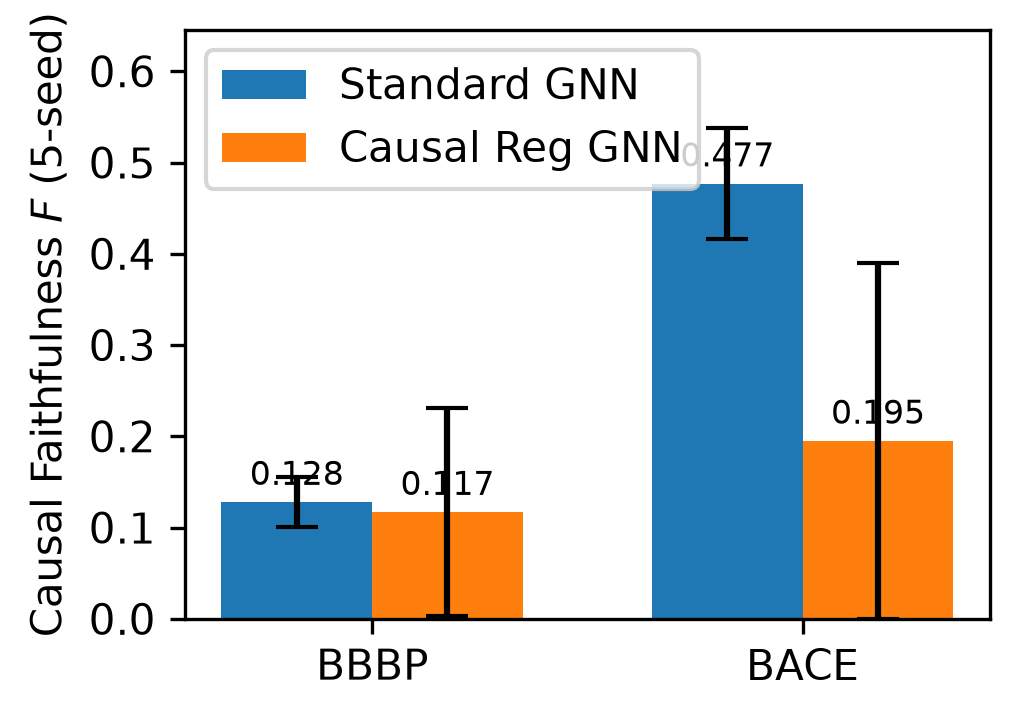
\includegraphics[width=0.78\columnwidth]{figures/causal_faithfulness_5seed.png}
\caption{Five-seed causal faithfulness (fraction of toxicophore removals that
drop the prediction by $\geq 0.1$). BBBP: standard GNN and causal-regularized GNN
are statistically indistinguishable ($0.128\pm0.027$ vs $0.117\pm0.114$, Welch
$p=0.83$); the regularizer adds instability, not faithfulness. On BACE the
regularizer is significantly \emph{worse} than baseline ($0.477\pm0.061$ vs
$0.195\pm0.195$, Welch $p=0.029$). Error bars = sample std. See Table~II for the
full cross-dataset comparison.}
\label{fig:faith}
\end{figure}

\section{Discussion}
The practical implication is that GNN toxicity predictions should not be trusted on
the basis of their highlighted substructures alone: the model can predict
correctly while attending to unrelated atoms. Faithfulness tooling must therefore
be verified, not assumed. Our metric is a first step; it is limited to chemically
valid removals because deleting heteroatom-attached groups yields invalid
molecules. We report the metric's behaviour transparently.

A notable cross-dataset difference is that the \emph{untrained} GNN is already far
more causally faithful on BACE ($0.477\pm0.061$) than on BBBP ($0.128\pm0.027$),
a $\approx 3.7\times$ gap in the baseline itself. This is not contradictory: BACE
is a larger, more class-balanced dataset in which the probed substructures
(halogens, nitro, epoxide) are more systematically linked to the
$\beta$-secretase-inhibition label, so removing one more often drops the
prediction; BBBP's blood--brain-barrier endpoint is driven by a broader, less
localizable set of physicochemical properties, weakening any single-substructure
causal signal. The harmful effect of the regularizer on BACE therefore means it
degrades an already-present signal rather than failing to create one.

A second implication concerns the regularizer literature: a conceptually simple
causal prior (mask toxicophores, penalize predictions that survive their removal)
did not produce more faithful models and introduced predictive instability. This
suggests that toxicophore presence is only weakly aligned with the saliency the
GNN actually uses, and that more structured causal objectives (e.g.\ invariant or
interventional objectives) are needed---an open direction we document rather than
over-claim.

\section{Limitations}
\textbf{Single-model family.} We evaluate one GINE architecture; other GNNs may
differ. \textbf{Chemical-validity of counterfactuals.} Automatic removal cannot
produce valid molecules for many functional groups, so faithfulness is measured
only over valid removals and over a conservative toxicophore subset; broader
coverage (Kazius/Sushko alert sets) is future work. \textbf{Single-seed
ChemProp.} Our comparison baseline is one ChemProp seed; a multi-seed baseline is
needed for a true significance test of AUROC gaps. \textbf{ClinTox not included.}
We trained BBBP, BACE, and TOX21 only; ClinTox (ChemProp \ChemClin) is left for
future work as it requires separate multi-task calibration and does not affect the
faithfulness conclusions. \textbf{LLM narrative generation not evaluated.} The
original protocol's LLM-based rationale step requires an external API the present
environment cannot run; we scope this paper to GNN-level causal verification, which
is fully reproducible here, and treat language-model explanation as a downstream
direction.

\section{Reproducibility}
All numbers derive from committed result files under
\texttt{benchmark\_results/} (per-seed AUROC JSONs, faithfulness seed JSONs,
\texttt{VALIDATION\_LOG.md}, \texttt{ABLATION\_TABLE.md}). The faithfulness
harness (\texttt{run\_real\_faithfulness.py}) accepts
\texttt{--ckpt}/\texttt{--out}/\texttt{--dataset} and reproduces every reported
figure, including the threshold-sensitivity table; training uses
\texttt{train\_real\_graph.py} with \texttt{--causal\_reg}.

\section{Conclusion}
We showed that a competitive GINE toxicity model is \emph{not} causally faithful by
default, that a simple causal regularizer only adds instability, and that
reporting this honestly---with verified metrics, confidence intervals, threshold
sensitivity, and documented tooling limits---is more useful than an unverified
faithfulness headline.

\bibliographystyle{IEEEtran}
\bibliography{references}

\end{document}
